\documentclass{beamer}

\usepackage{beamer_tom}
\graphicspath{{./images/}}
%\usepackage{natbib}

\usepackage{bibentry}

\def\keypoint#1{\hfill\textcolor{gray}{#1}}
\def\mycite#1{\keypoint{\normalsize\cite{#1}}}
\def\tT{\widetilde{T}}


\newcommand{\parttitleframe}[1]{
    \begin{frame}[t]
    \vskip5em
    \centering
    \begin{beamercolorbox}[sep=8pt,center,shadow=true,rounded=true]{title}
        \usebeamerfont{title}\insertsectionhead%
    \end{beamercolorbox}
    \vskip5em
    \begin{block}{References}
        \small\vskip.5em
        
        \begin{itemize}
            \item\bibentry{#1}
        \end{itemize}
    \end{block}
    \end{frame}
}


\institute{\\Parietal -- INRIA Saclay}
\author{Thomas Moreau}
\title{
	Learning Recurring Patterns\\in Large Signals with\\Convolutional Dictionary Learning
}
\collaborators{T. Dupré la Tour (Telecom), M. Jas (Telecom),\\
               A. Gramfort (INRIA), N. Vayatis (CMLA), L. Oudre (UP13)}

\date{
    January 24, 2019
}

\setbeamertemplate{title page}[frame]
\def\extraLogo{}

\usepackage[titlenumbered,ruled,noend]{algorithm2e}

\begin{document}

	\begin{frame}
		\titlepage
        
        \nobibliography{library}
	\end{frame}

	\begin{frame}{Studying brain activity through electromagnetic signals}
	\begin{itemize}
		\item Brain (electrical) activity produces an electromagnetic field.
		\item This can be measured with EEG or MEG.
	\end{itemize}

	\begin{columns}[T]
		\column{.5\textwidth}
	\centering
	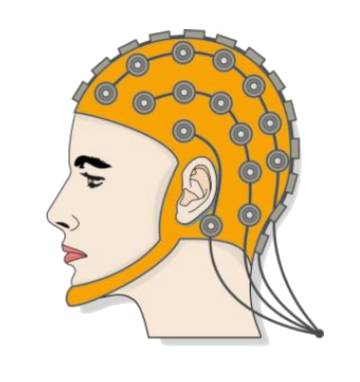
\includegraphics[height=6em]{eeg}\hskip4em
	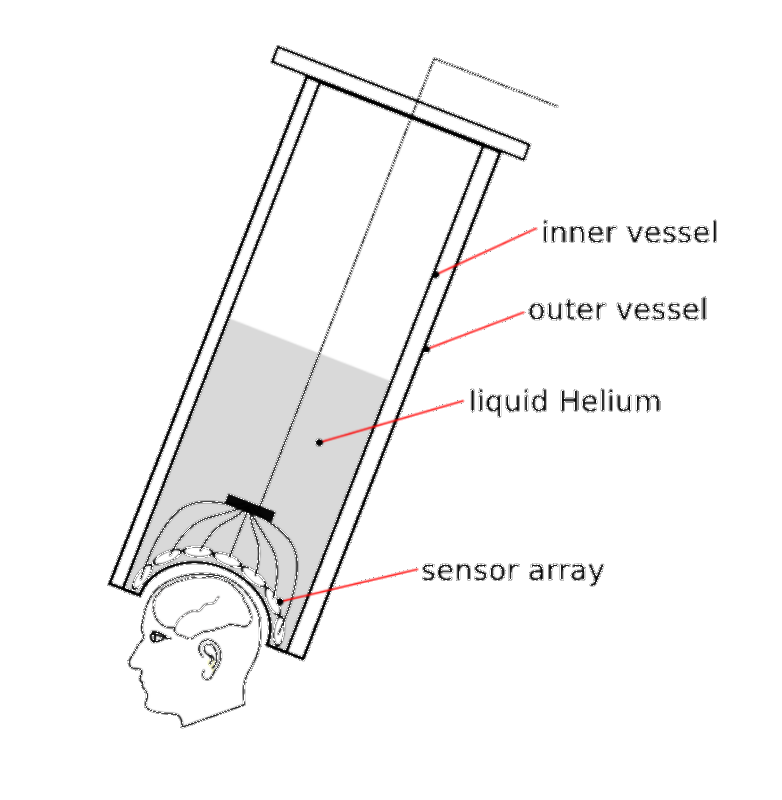
\includegraphics[height=6em]{meg}\\
	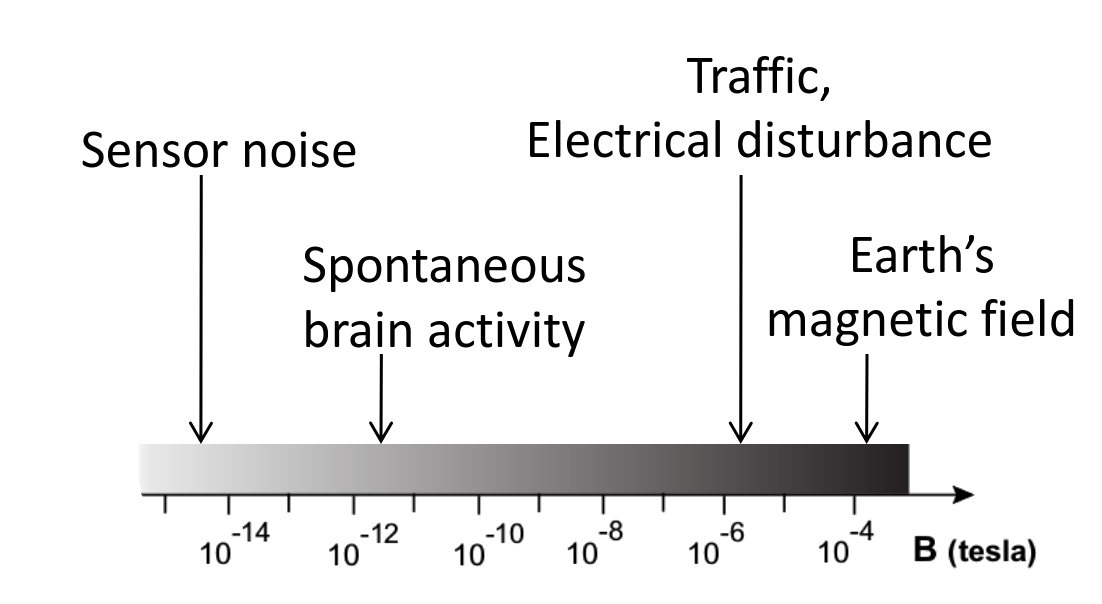
\includegraphics[height=8em]{scale_electro}
	\column{.5\textwidth}
	\vskip3em
	\hskip2em
	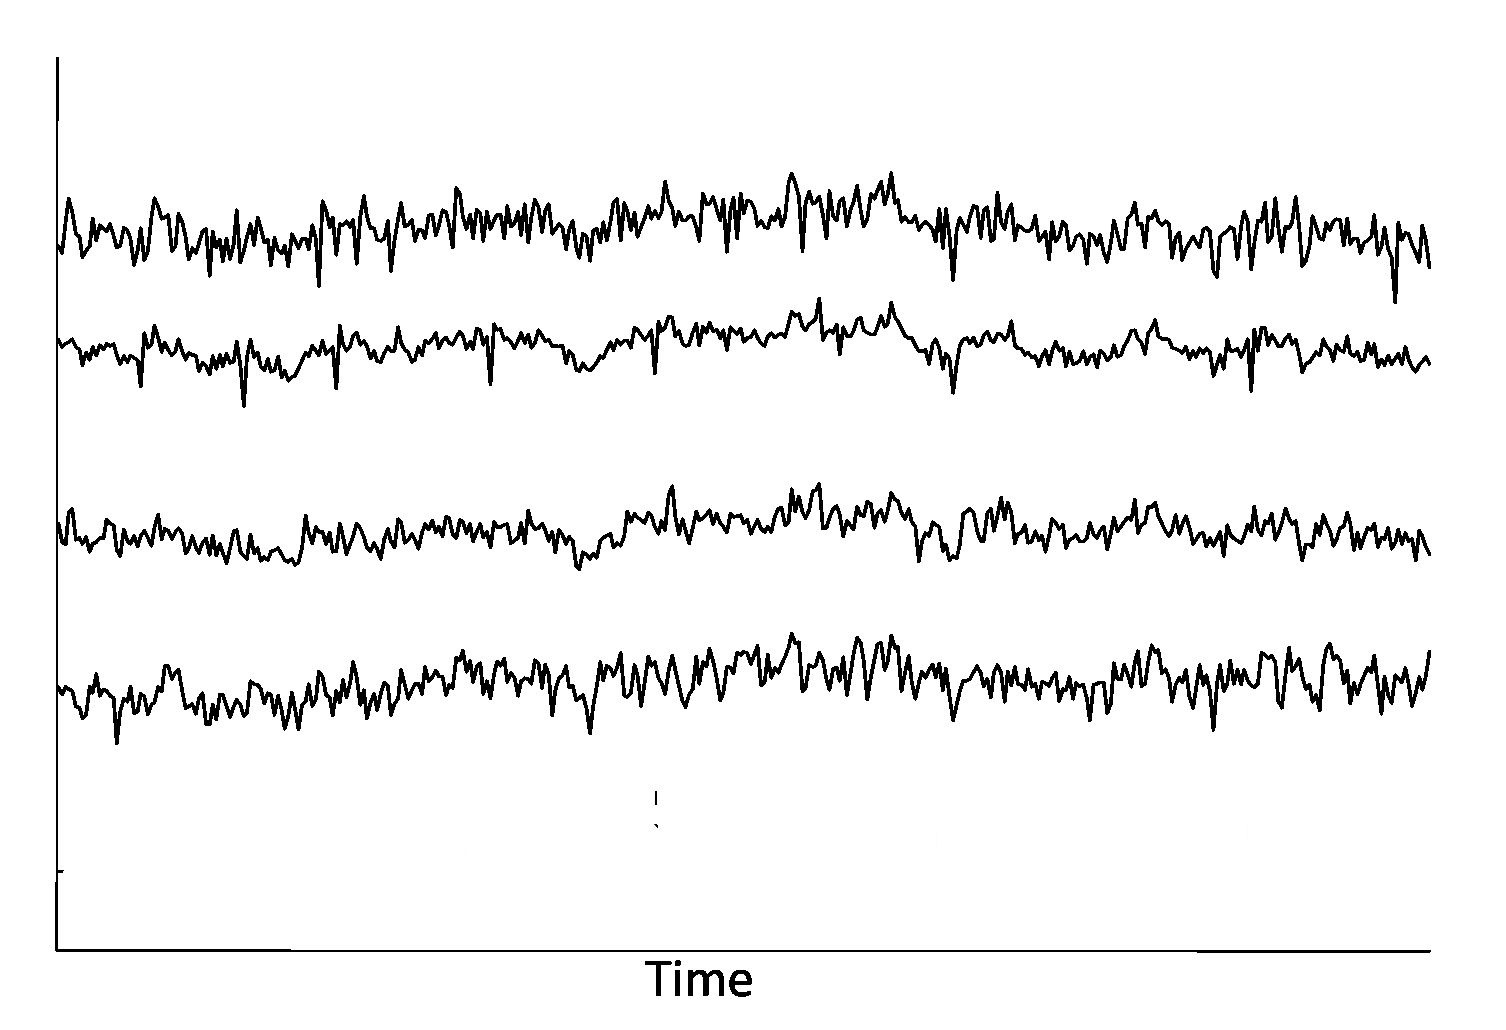
\includegraphics[height=8em]{multivariate_eeg}
	\end{columns}
	\end{frame}
	
\begin{frame}{Goal: Study Oscillation in Neural Data}
	
    \textbf{}Oscillations are believed to play an important role in cognitive functions.\\[3em]
	Many studies rely on Fourier or wavelet analyses:\\[.5em]
	\begin{itemize}\itemsep1em
		\item Easy interpretation,
		\item Standard analysis \eg{} canonical bands alpha, beta or theta.\\\mycite{buzsaki2006rhythms}
	\end{itemize}

\end{frame}

\begin{frame}{Goal: Study Oscillation in Neural Data}

		However, some brain rhythms are not sinusoidal, \eg mu-waves\mycite{hari2006action}\\
		\hskip5em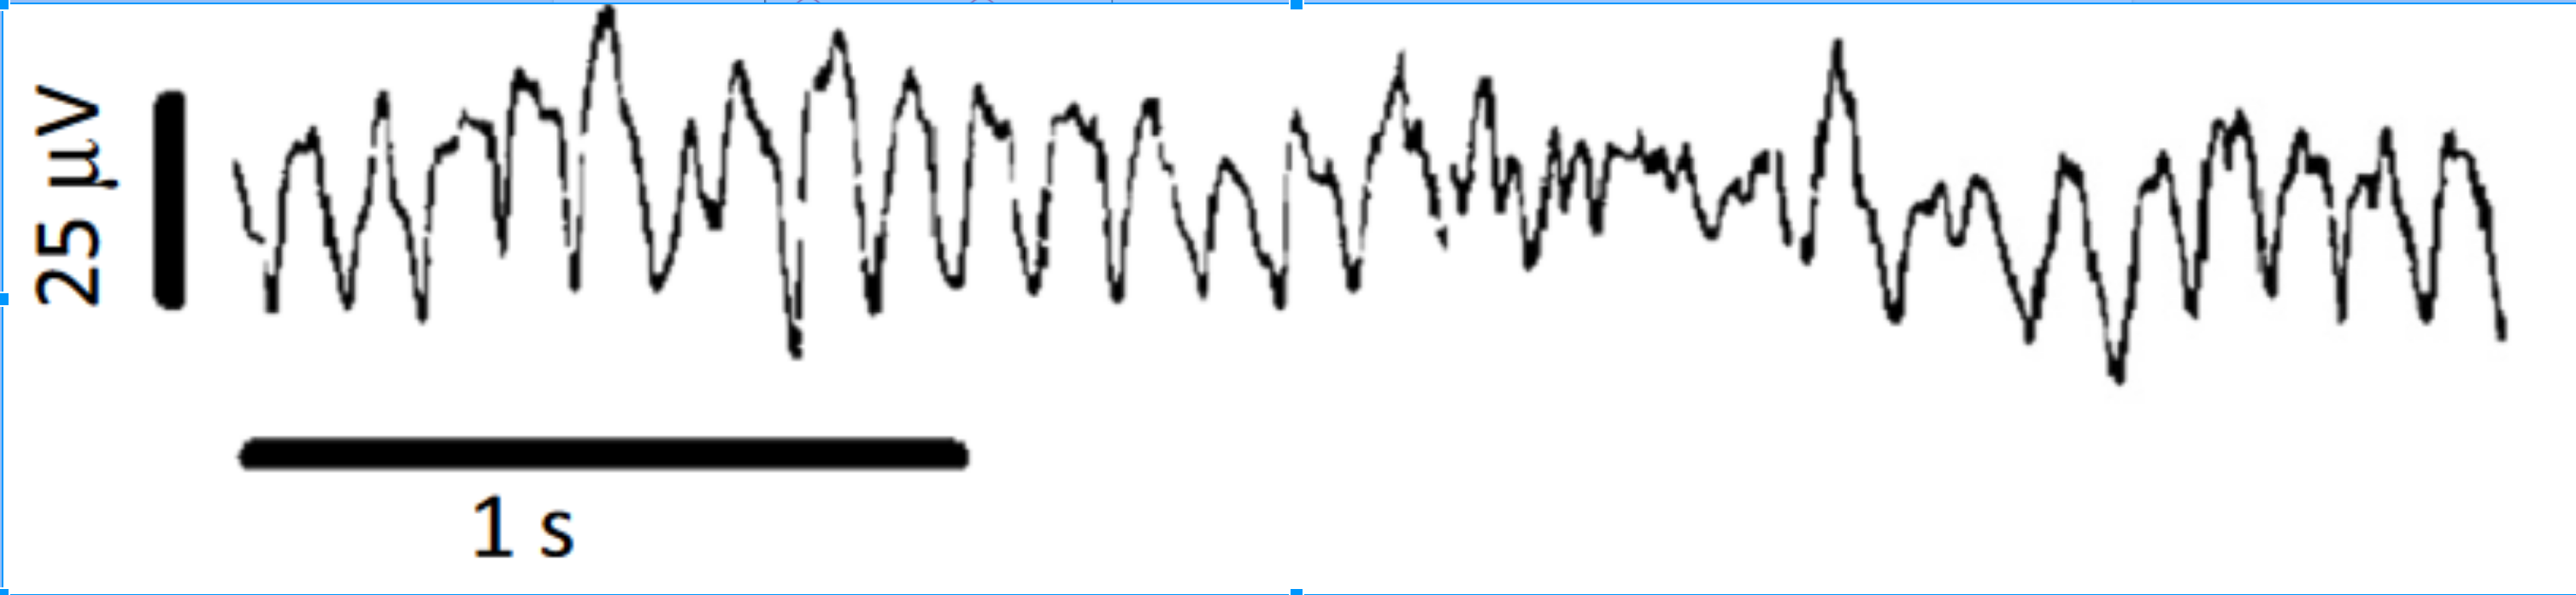
\includegraphics[width=.7\textwidth]{waveform}\\
		and filtering degrades waveforms\\
		\hskip8em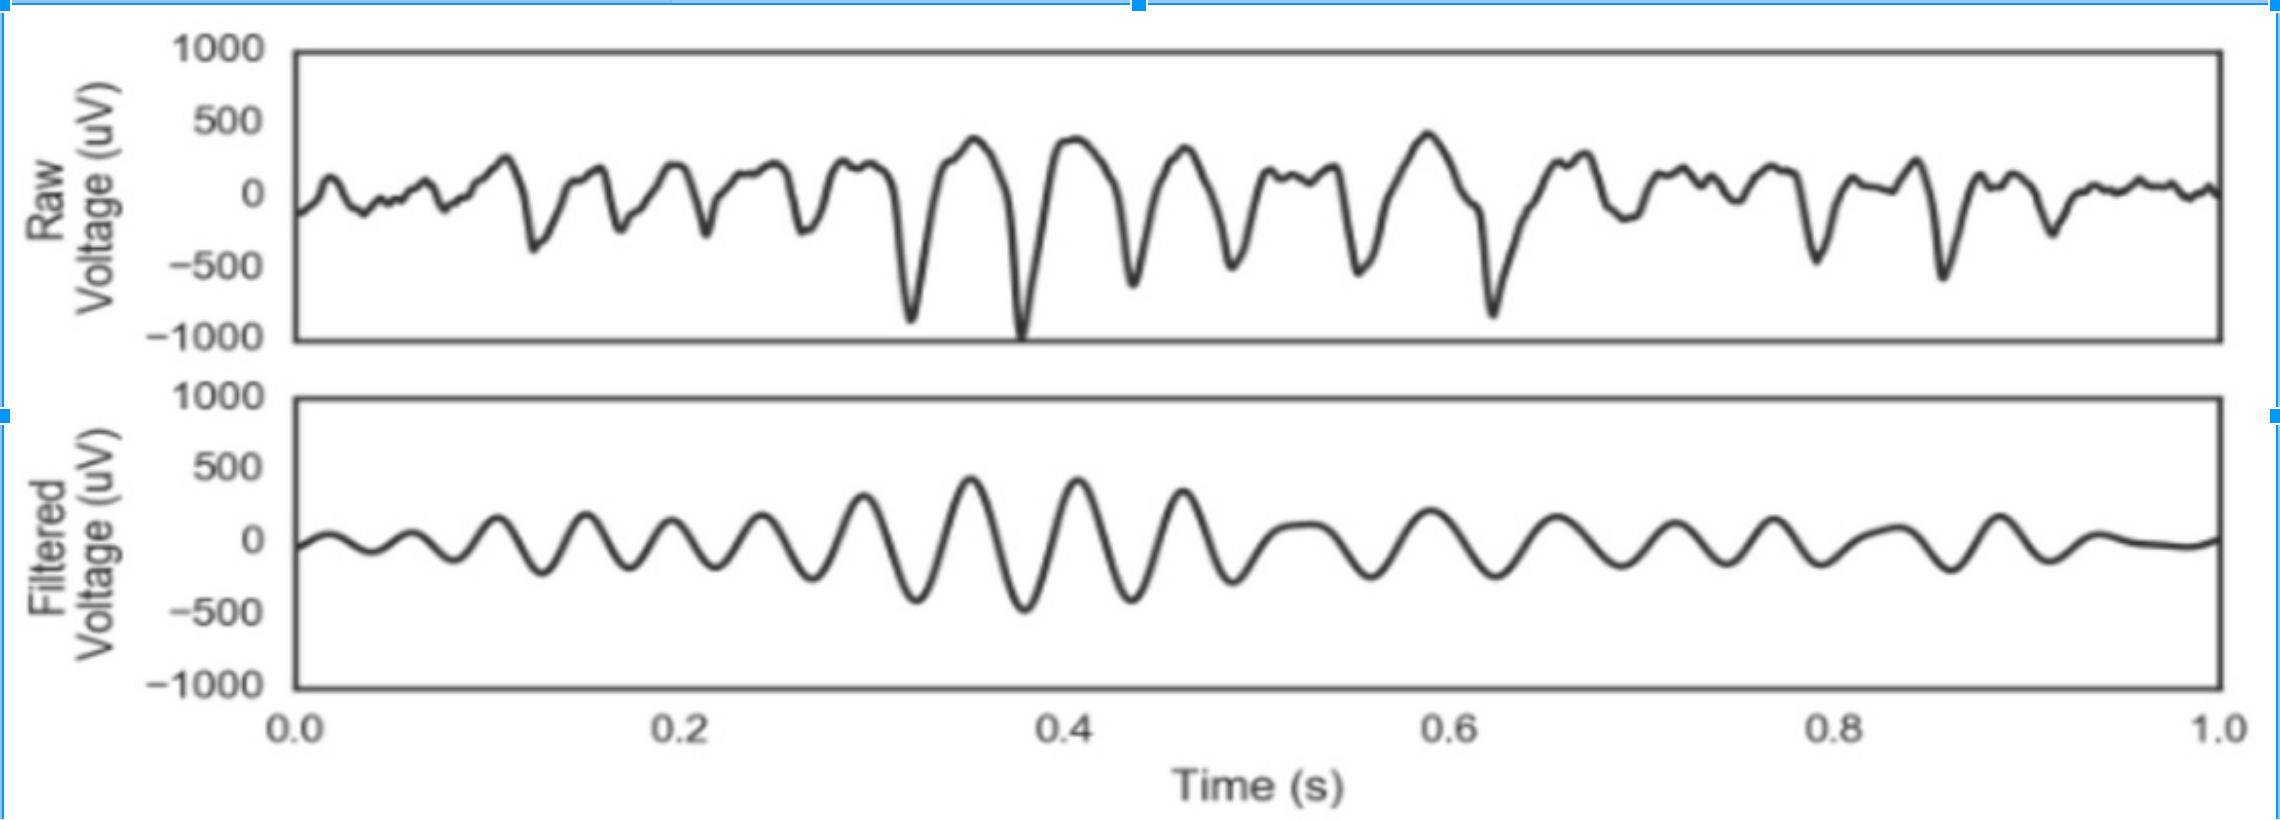
\includegraphics[width=.5\textwidth]{filtering_brain}


	\strongpoint{Can we do better with data-driven approach?}
\end{frame}


\begin{frame}{Extracting shift invariant patterns}
	\textbf{Key idea}: decouple the localization of the patterns and their shape
	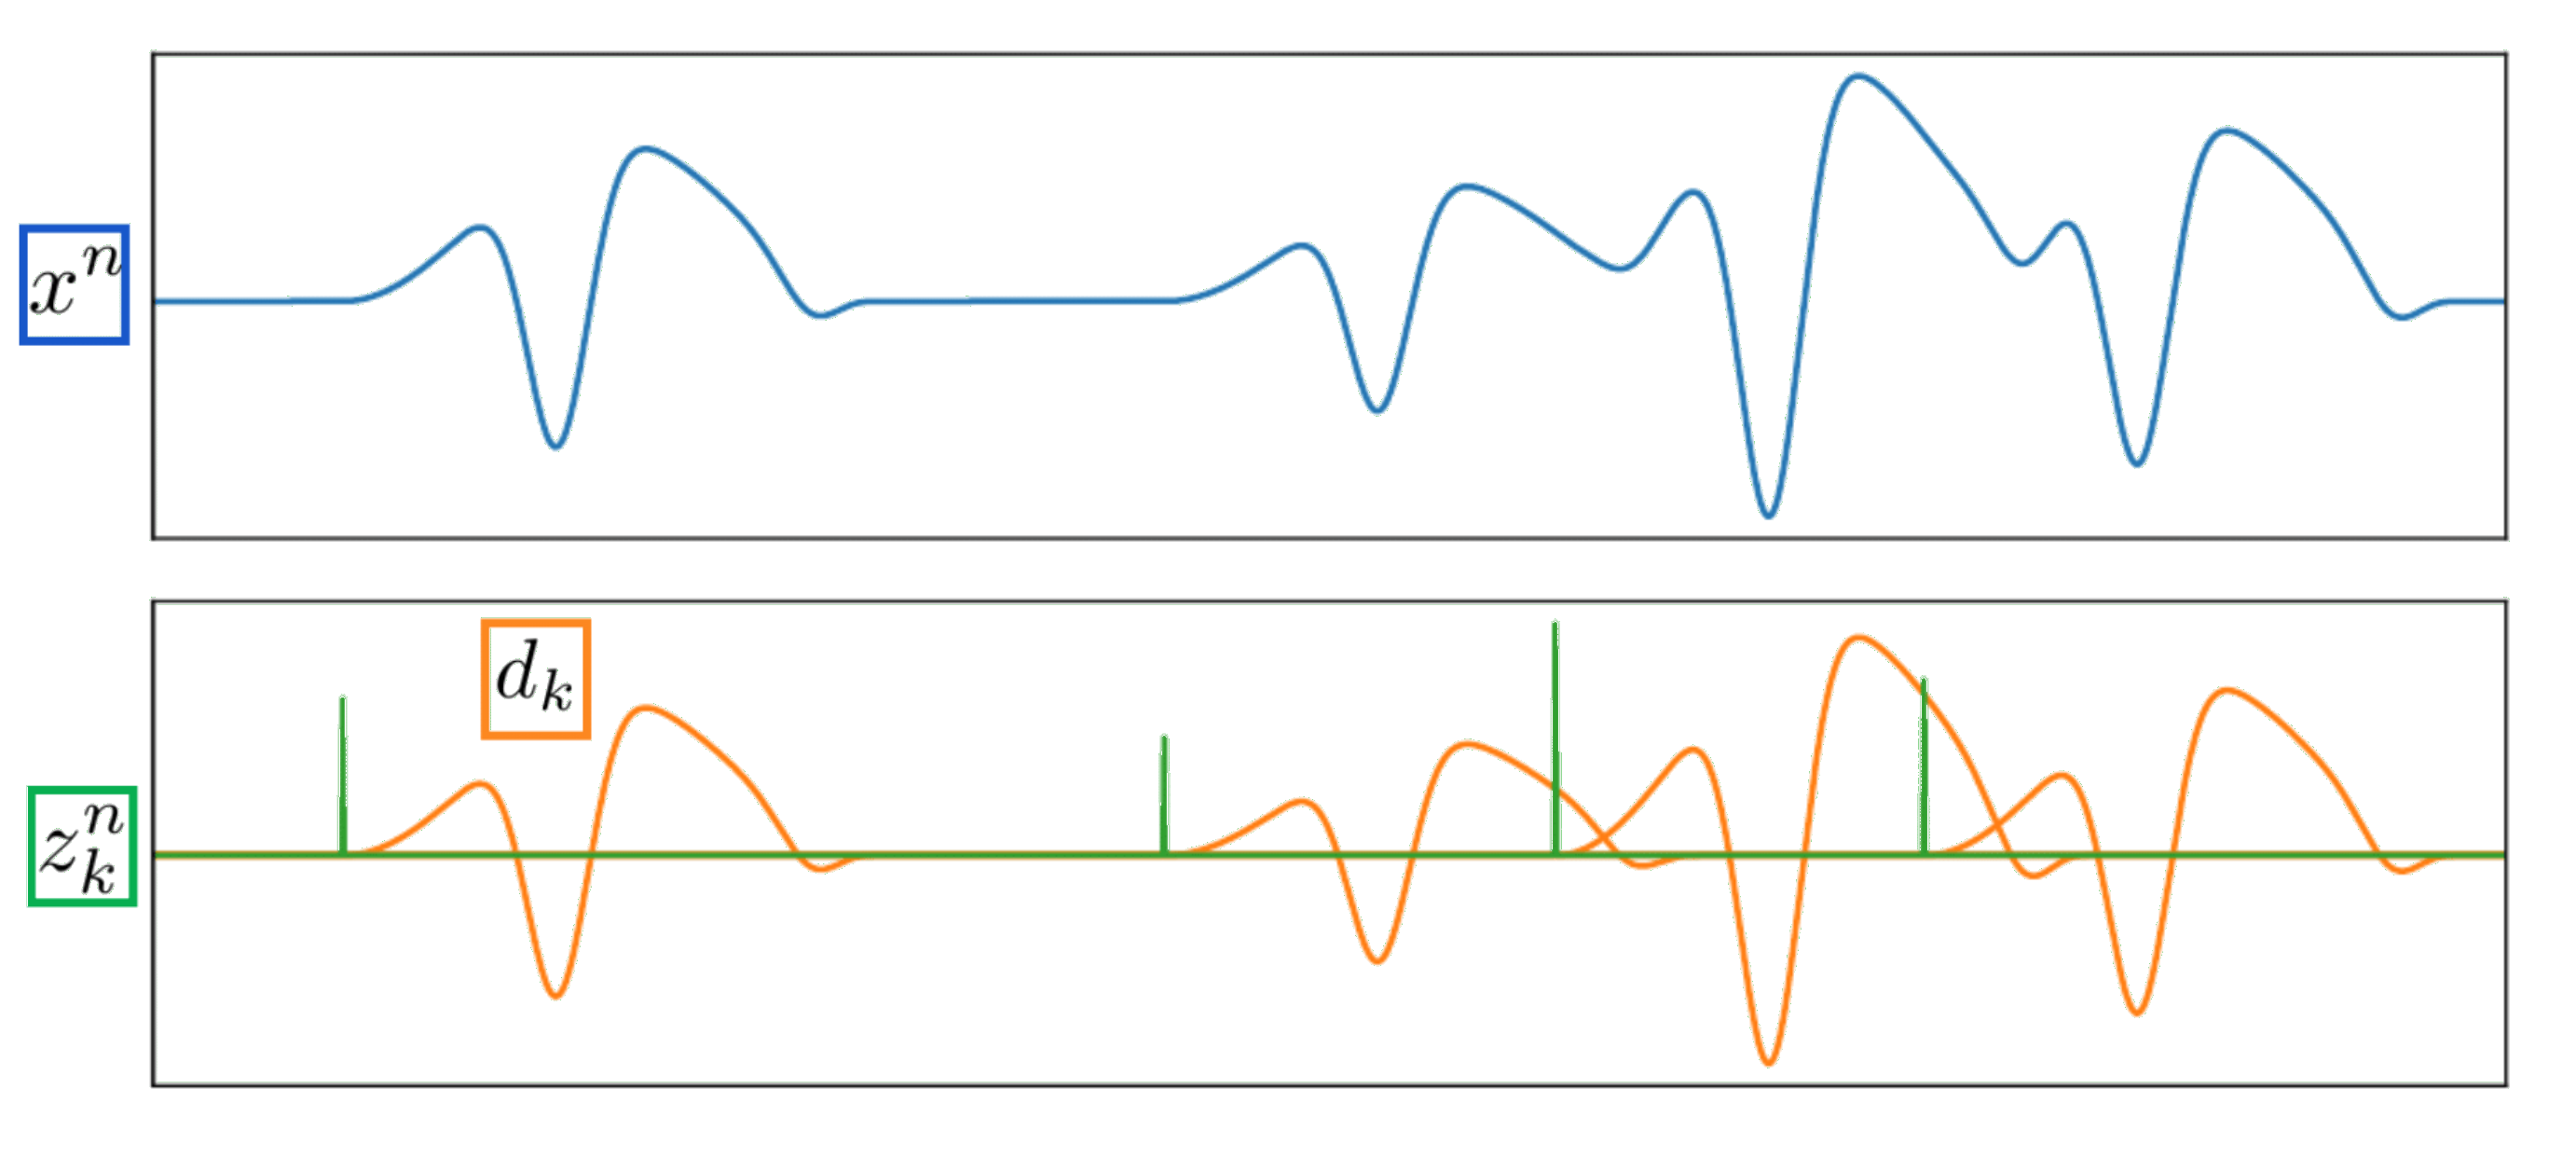
\includegraphics[width=\textwidth]{csc_explain_color.png}
	\only<2>{
        \vskip-2em
        \begin{columns}[T]
            \column{.3\textwidth}\vskip2em\centering\textbf{Convolutional\\Representation:} %
             \column{.7\textwidth}\centering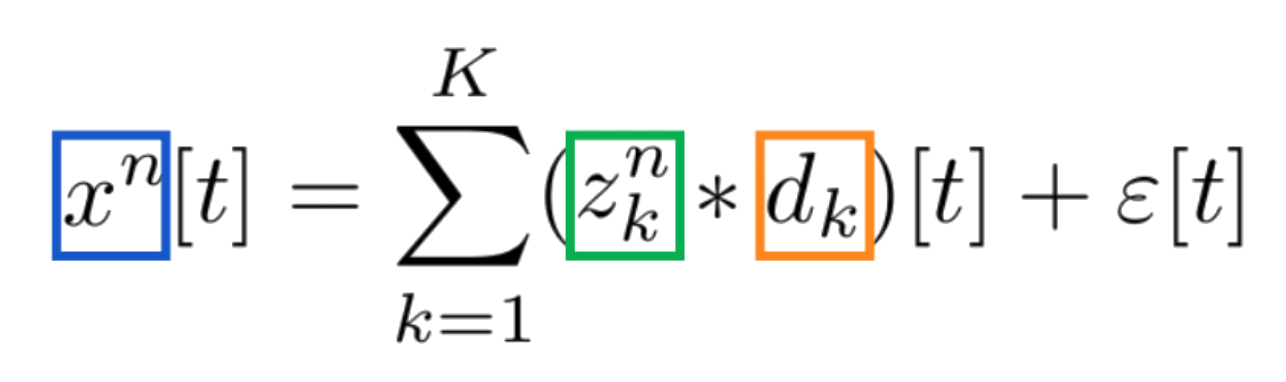
\includegraphics[width=.7\textwidth]{eq_csc_explain_color}
         \end{columns}
    }
	\uncover<3>{
        \vskip-2em
        \begin{columns}[T]
            \column{.3\textwidth}\vskip2em\centering\textbf{Convolutional Dictionary Learning:} %
            \column{.7\textwidth}\vskip-.5em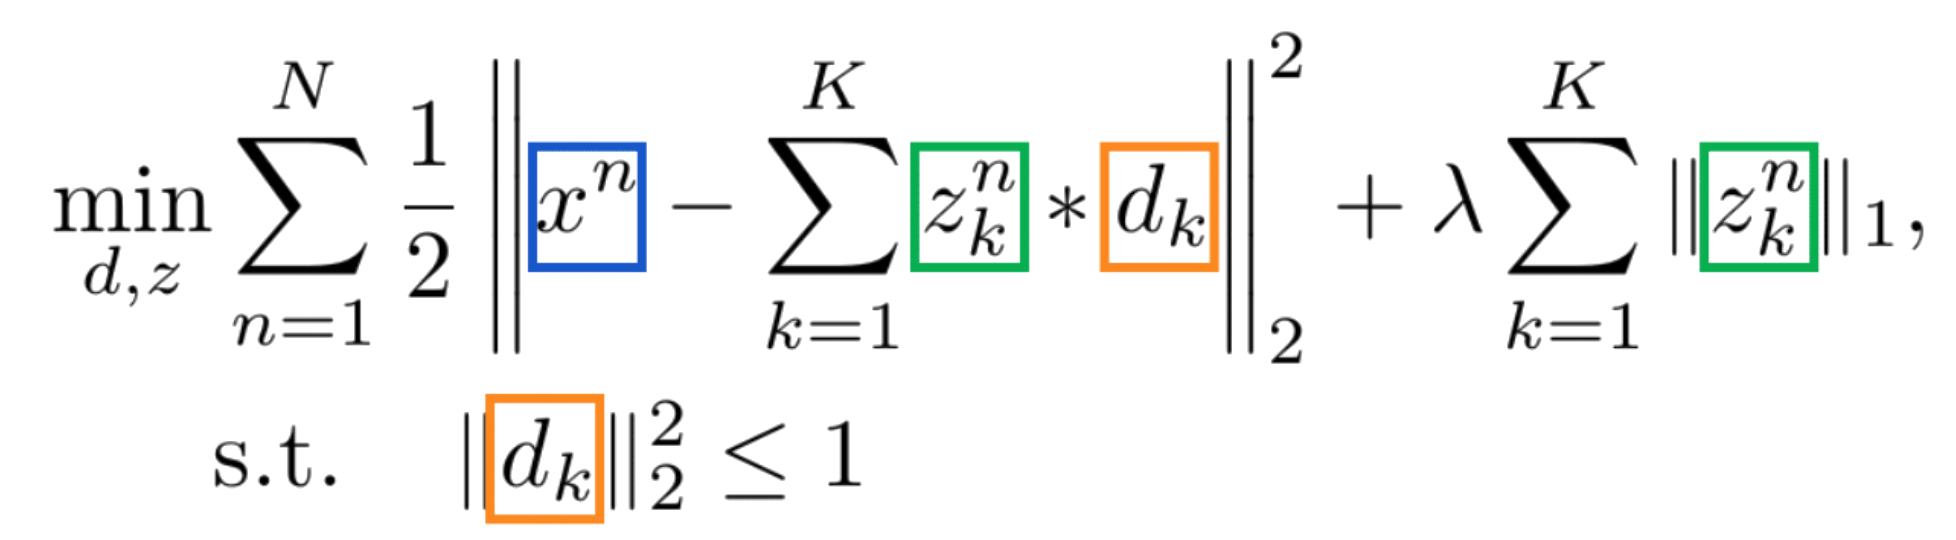
\includegraphics[width=\textwidth]{csc_eq_l1}
        \end{columns}
    }
\end{frame}


\begin{frame}{Shift-invariant Patterns in images}
\centering
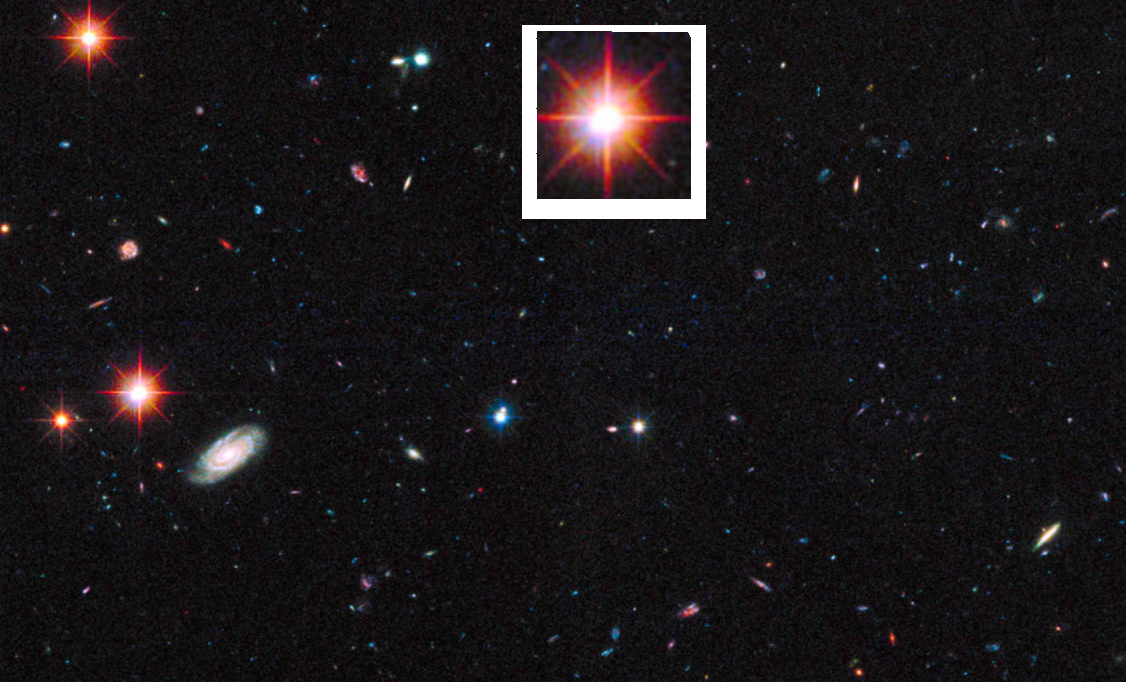
\includegraphics[height=.7\textheight]{cosmostat}\\[1em]
Images also have shift-invariant patterns that we might want to detect.
\end{frame}

\begin{frame}{Convolutional Dictionary Learning}

\textbf{\large Convolutional Dictionary Learning (CDL)}\mycite{Grosse2007}\\
For a set of $N$ univariate signals $x^n$, solve
\begin{equation}
    \label{eq:csc}
    \min_{d_k, z_k^n} \sum_{n=1}^N  \frac{1}{2}\|x^n - \sum_{k=1}^K z_k^n * d_k\|_2^2
                                    + \lambda\sum_{k=1}^K\|z^n_k\|_1
\end{equation}
\vskip1em
\textbf{Hypothesis:} patterns $d_k$ are not present everywhere in the signal. They are localized in time.
\strongpoint{Sparse activation signals $z$}
\vskip2em
\textbf{Extra hypothesis:} the patterns are in the $\ell_2$-ball: $\|d_k\|_2^2 \le 1$.
\end{frame}


\begin{frame}{Optimization strategy}
The problem \autoref{eq:csc} is not jointly convex in $z^n_k$, and  $d_k$ it is convex in each block of coordinate.\\[1em]

\textbf{Alternate minimization} (\emph{a.k.a.} Bloc Coordinate Descent):\\[.5em]

\begin{itemize}\itemsep1em
    \item \textbf{Z-step:} given a fixed estimate of the atom, compute the activation signal $z^n_k$ associated to each signal $X^n$.
    \item \textbf{D-step:} given a fixed estimate of the activation, update the atoms in the dictionary $d_k$.
\end{itemize}
\end{frame}


\section{Convolutional Sparse Coding with Locally Greedy Coordinate Descent (LGCD)}
\parttitleframe{Moreau2018}

\begin{frame}{Convolutional Sparse Coding}

$N$ independent problem such that
\[
\label{eq:sparse_code}
\min_{z_k^n}  E(z^n) = \frac{1}{2} \left\|x^n - \sum_{k=1}^K z_k^n * d_k\right\|_2^2
+ \lambda\sum_{k=1}^K\left\|z_k^n\right\|_1~.
\]
\vskip.5em
This problem is convex in $z_k$ and can be solved with different techniques:
\begin{itemize}\itemsep.5em
\item Greedy CD \mycite{Kavukcuoglu2013}
\item Fista \mycite{Chalasani2013}
\item ADMM \mycite{Bristow2013}
\item L-BFGS \mycite{Gramfort2017}
\end{itemize}

\strongpoint{These methods can be slow for long signals as the complexity of each iteration is at least linear in the length of the signal.}

\end{frame}

\begin{frame}{Greedy coordinate descent (GCD)\mycite{Kavukcuoglu2013}}

For the Greedy Coordinate Descent, only 1 coordinate is updated at each iteration:

\vskip.5em
\begin{enumerate}\itemsep1em
\item The coordinate $z_{k_0}[t_0]$ is updated to its optimal value $z'_{k_0}[t_0]$ when all other coordinate are fixed:
\[
z'_{k}[t] =  \max\left(\frac{\beta_{k}[t] - \lambda}{\| d_{k}\|_2^2}, 0\right) ,
\]
with $\beta_{k}[t] = \left[\left(X- \sum_{l=1}^K z_l * d_l +z_{k}[t]e_t* d_{k}\right)
                           * d_{k}^\Lsh \right][t]$
\item Greedy coordinate selection:
\[
    (k, t) = \argmax_{(k ,t)} |z_k[t] - z'_k[t]|
\]
\end{enumerate}

\end{frame}



\begin{frame}{Locally greedy coordinate descent (LGCD) \mycite{Moreau2018}}


We introduced the LGCD method which is an extension of GCD.\\
{
    \centering
    \inputTikZ{.7}{LGCD}
}

\only<1-2>{
    \vskip1em
    GCD has $\mathcal O(KT)$ computational complexity.\\[1em]
    \only<2>{But the update itself has complexity $\mathcal O(KL)$}
}

\visible<3->{
With a partition $\mathcal C_m$ of the signal domain $\interval{1, K}\times\interval{0, T}$,
\[
\mathcal C_m = \interval{1, K}\times\interval{\frac{(m-1)\tT}{M}, \frac{m\tT}{M}}
\]%
}%
\visible<4->{%
The coordinate to update is chosen greedily on a sub-domain $\mathcal C_m$\\[1em]

{\centering$\mathcal O$(Coordinate selection) = $\mathcal O$(Coordinate Update)\\[1em]}

The overall iteration complexity is $\mathcal O(KL)$ instead of $\mathcal O(KT)$.
\strongpoint{Efficient for sparse $Z$}
}


\end{frame}

\begin{frame}{Fast optimization}
    Comparison of the coordinate selection strategy for CD on simulated signals\\
    We set $K=10$, $L=150$, $\lambda = 0.1 \lambda_{\max}$\\[1em]
    \centering
    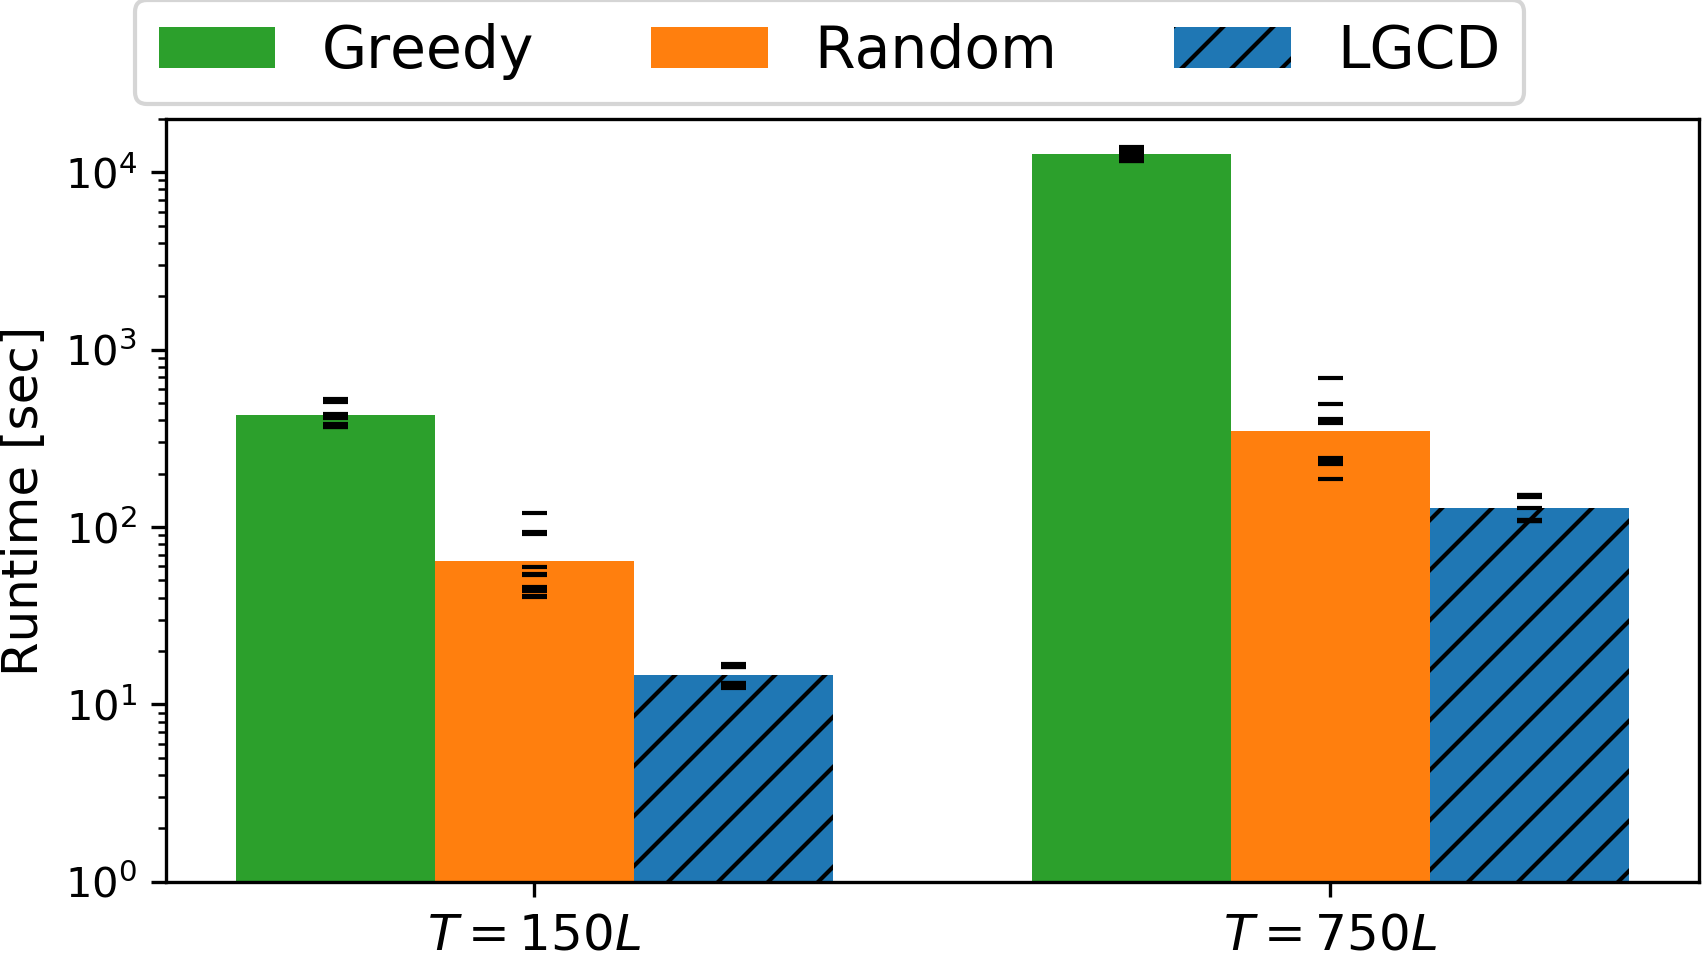
\includegraphics[width=.9\textwidth]{CD_strategies_comparison.png}
\end{frame}


\section{Distributed optimization for CSC}

\parttitleframe{Moreau2019}


\begin{frame}{Weak dependence of the coordinate updates}
	The update of the $W$ coordinates $(k_w, \omega_w)_{w=1}^W$ with additive update $\Delta Z_{k_w}[\omega_w]$ changes the cost by:
\begin{align*}
\Delta E =
\overbrace{\sum_{i=1}^W\Delta E_w}^{
    \text{iterative steps}}
- \underbrace{\sum_{w \neq w'}(d_{k_w} * d_{k_{w'}}^\Lsh)[\omega_{w'} - \omega_w]
    \Delta Z_{k_w}[\omega_w] \Delta Z_{k_{w'}}[\omega_{w'}]}_{
    % \Delta Z_{k_w}[w] \Delta Z_{k_{w'}}[w']}_{
    \text{interference}}, \label{eq:interf}
\end{align*}

\strongpoint{If the updates are far enough, they can be considered as independent.}
\end{frame}

\begin{frame}{Distributed Convolutional Coordinate Descent (DICOD)}

{
    \centering
    \inputTikZ{.7}{DICOD}\\
}
\vskip1em
    \begin{itemize}[<+->]\itemsep.5em
        \item Split the coordinates in continuous sub-segment
        $\mathcal S_w = \left[\frac{(w-1)T}{W}, \frac{wT}{W}\right[$.
        \item Use Greedy updates in parallel in each sub-segment.
        \item Notify neighbor workers when the update is on the border of $\mathcal S_w$.
    \end{itemize}

    \visible<4>{
    \vskip2em
    This algorithm converges to the solution of the CSC for 1D signals but not for higher dimension signals such as images.}
\end{frame}


\begin{frame}{Distributed Convolutional Dictionary Learning (DiCoDiLe-Z)}

\begin{itemize}\itemsep1em
    \item Extension of DICOD for high dimensional signals.
    \item Use LGCD locally in each workers (better iteration complexity). 
    \item Use Soft-locks to avoid interference (ensure convergence).
\end{itemize}
\end{frame}


\begin{frame}{Distributed Convolutional Dictionary Learning (DiCoDiLe-Z)}
\vskip1em
    \begin{columns}[c]
    \column{.35\textwidth}
    \begin{itemize}\itemsep1em
        \only<1>{
            \item Update candidate $\omega_0$ is independent of other workers as
            \[
                \mathcal V(\omega_0) \subset \mathcal S_w
            \]
        }
    
        \only<2>{
            \item Update candidate $\omega_1$ impacts $\mathcal S_{w+1}$
            \[
                \mathcal V(\omega_1) \not\subset \mathcal S_w
            \]
            \item It is accepted only is no better update is possible in the "soft-locked" area.
            \item Need to notify $\mathcal S_{w+1}$.
        }
        \only<3>{
            \item Updates in $\omega_2$ need to notify worker $w$ to maintain consistent estimate in the border zone $\mathcal B_L(\mathcal S_w)$.
            
            \item Low communication: decentralized and below 1ko.
        }
       \end{itemize}
    \column{.65\textwidth}
        \inputTikZ{.75}{Sw_dicod.tex}
    \end{columns}
\end{frame}



\begin{frame}{Numerical speed-up}

\centering
        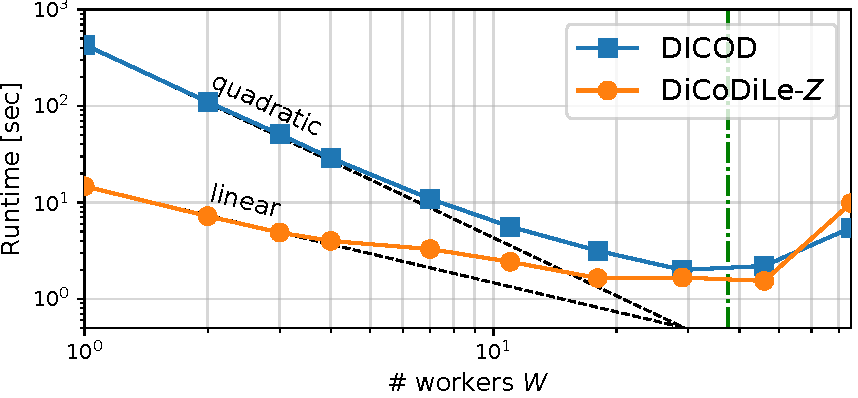
\includegraphics[width=\textwidth]{scaling_T150}
    \\
    \large Running time as a function fo the number of workers $W$.

\end{frame}

\section{Rank-1 Constrained Convolutional Dictionary Learning}

\parttitleframe{Dupre2018}

\begin{frame}{D-step: solving for the atoms}

The dictionary update is performed by minimizing
\begin{equation}
\min_{\|d_{k}\|_2 \leq 1} E(\{d_k\}_k) \overset{\Delta}{=} \sum_{n=1}^N\frac{1}{2}\|X^n - \sum_{k=1}^K z^n_k * d_k\|_{2}^{2} \hspace{6pt}
\enspace .
\end{equation}

Computing $\nabla_{d_k} E(\{d_k\}_k)$ can be done efficiently
\[
\nabla_{d_{k}} E(\{d_k\}_k)
= \sum_{n=1}^N (z_k^n)^\Lsh * \left(x^n - \sum_{l=1}^K z^n_l * d_l\right)
=  \Phi_k - \sum_{l=1}^K \Psi_{k, l} *  d_l \enspace ,
\]

\strongpoint{Save with Projected Gradient Descent (PGD) with an Armijo backtracking line-search for the d-step \mycite{Wright1999}.}

\end{frame}




\begin{frame}{How to extend CSC to multivariate signals?}
We can just use multivariate convolution,
\[
	\underbrace{X[t]}_{\in\Rset^P} = \sum_{k=1}^K \left(z_k * \pmb D_k\right)[t] = \sum_{k=1}^K \sum_{\tau=1}^L z_k[t-\tau] \underbrace{\pmb D_k[\tau]}_{\in \Rset^P}
\]
with:
\begin{itemize}
	\item $X$ a multivariate signal of length $T$ in $\Rset^P$
	\item $\pmb D_k$ a multivariate signal of length $L$ in $\Rset^P$
	\item $z_k$ a univariate activation signal of length $\tT = T - L + 1$
\end{itemize}
\vskip1em
However, this model does not account for the physics of the problem.
\end{frame}

\begin{frame}{EM wave diffusion}
	\begin{itemize}
		\uncover<1->{\item Recording here with 8 sensors}
		\uncover<2->{\item EM activity in the brain}
		\uncover<3->{\item The electric field is spread \textbf{linearly} and \textbf{instantaneously} over all sensors (Maxwell equations)}
	\end{itemize}
	\centering
	\only<1>{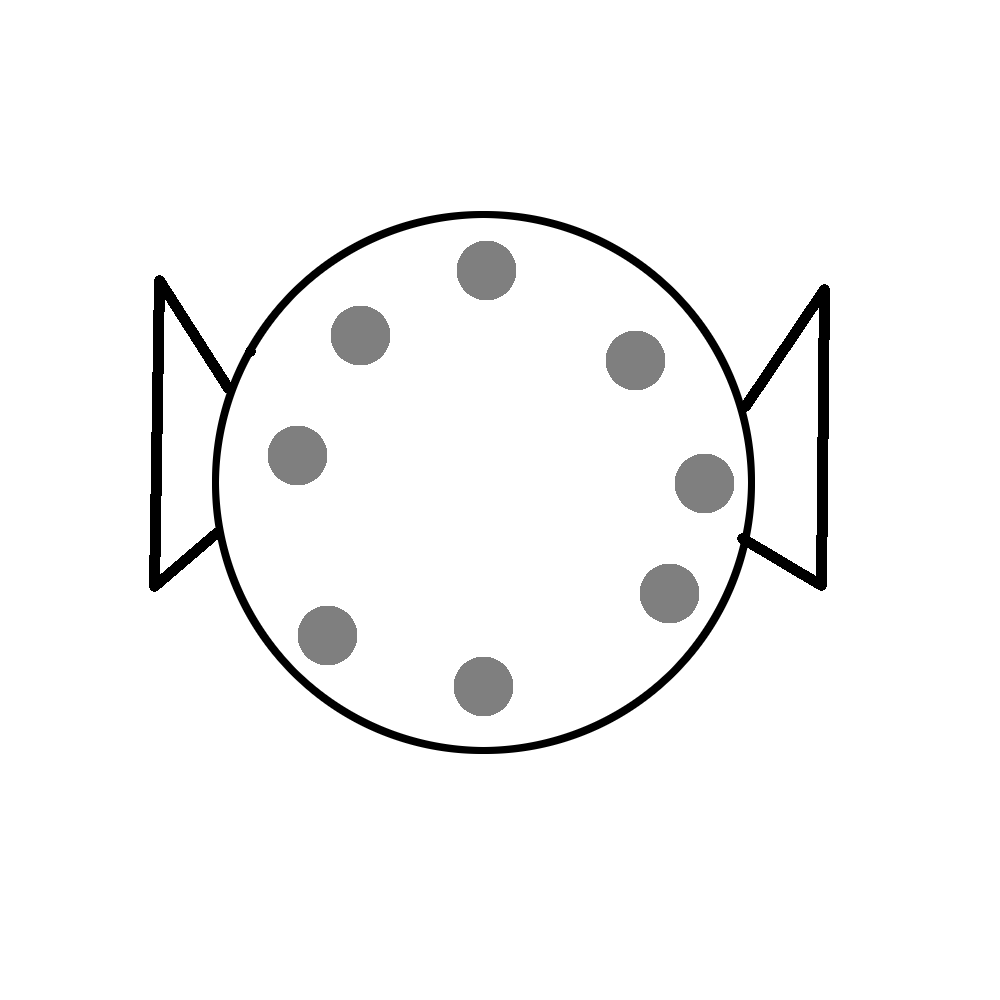
\includegraphics[width=.5\textwidth]{physic1}}%
	\only<2>{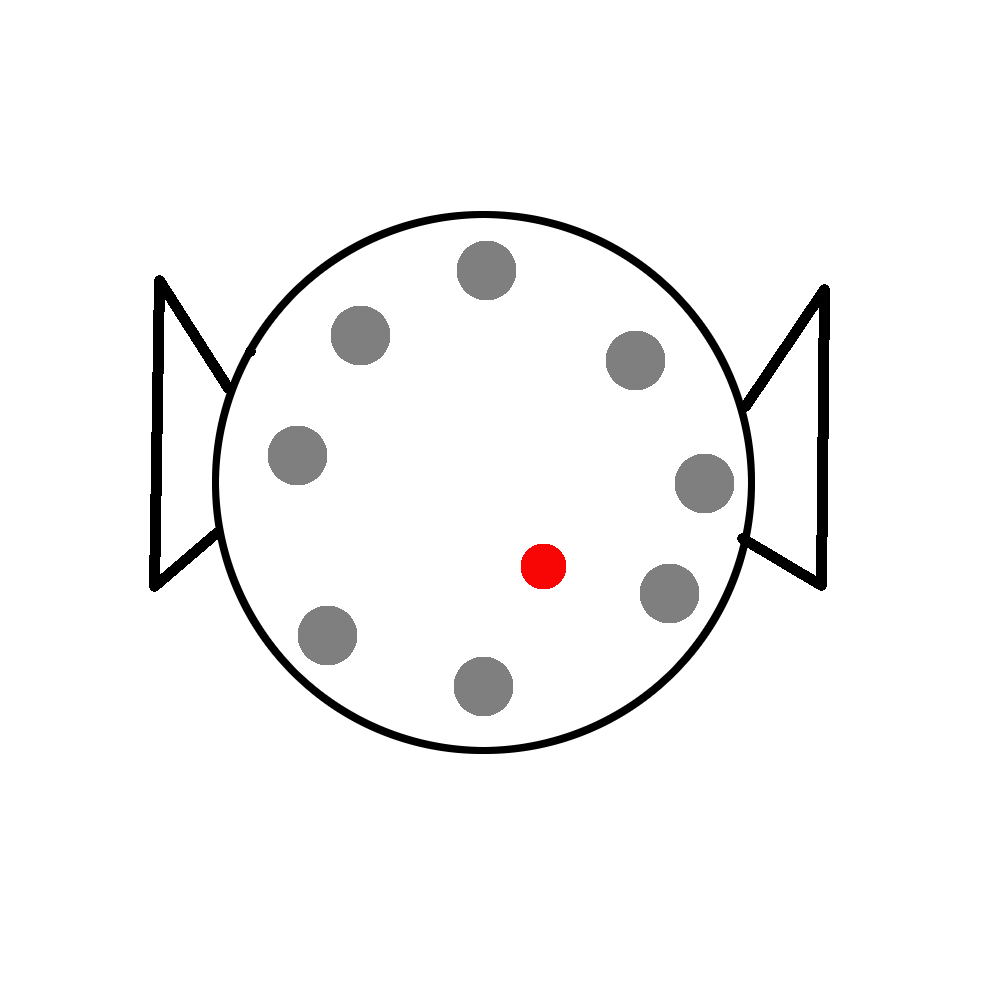
\includegraphics[width=.5\textwidth]{physic2}}%
	\only<3>{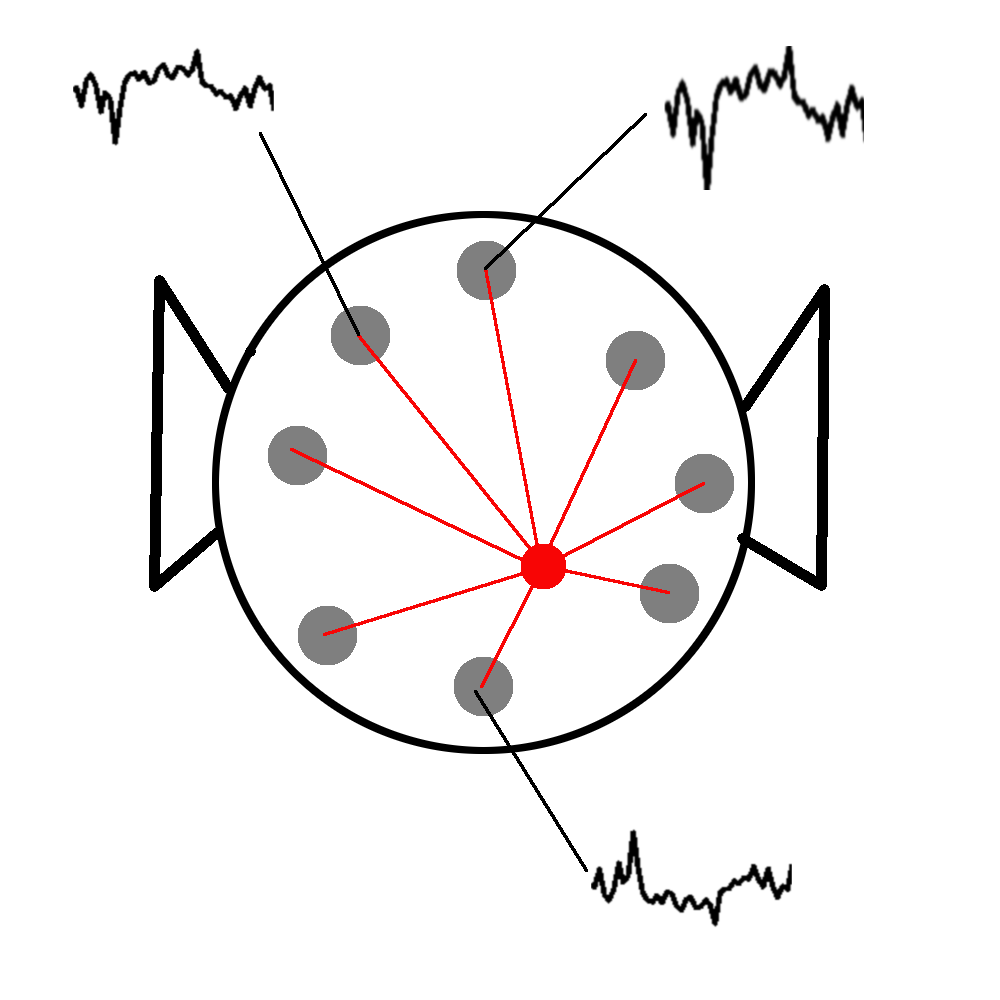
\includegraphics[width=.5\textwidth]{physic3}}
\end{frame}

\begin{frame}{Multivariate CSC with rank-1 constraint}
	\textbf{Idea}: Impose a rank-1 constraint on the dictionary atoms $D_k$
	\vskip1em
	To make the problem tractable, we decided to use auxiliary variables $u_k$ and $v_k$ \st{} $D_k = u_kv_k\top$.
	
	\begin{equation}
	\label{eq:multichannel_csc}
	\begin{split}
	\min_{u_k, v_k, z_k^n} &\sum_{n=1}^N\frac{1}{2}\left\|X^n - \sum_{k=1}^K z^n_k * (u_k^{ } v_k^\top)\right\|_{2}^{2}
	+ \lambda  \sum_{k=1}^K \left\|z^n_k\right\|_1, \hspace{6pt}\\
	&\text{s.t. } ~~ \|u_{k}\|_2^2 \leq 1 \text{  , }\|v_{k}\|_2^2 \leq 1 \text{  and } z_k^n \geq 0~.
	\end{split}
	\end{equation}
	
	Here,
	\begin{itemize}
		\item $u_k \in \Rset^P$ is the spatial pattern of our atom
		\item $v_k \in \Rset^L$ is the temporal pattern of our atom
	\end{itemize}
\end{frame}

\begin{frame}{Update in $u_k$ and $v_k$}

    The problem is not jointly convex in $u_k$ and $v_k$.\\[1em]
    Use an alternate minimization on these two blocks.\\[2em]
    
    The gradient can also be computed using sufficient statistics $\phi$ and $\psi$:
    \[
    \begin{split}
        \nabla_{u_k} E(\{u_k\}_k, \{v_k\}_k) &=  \nabla_{D_k}E(\{u_k\}_k, \{v_k\}_k) v_k
            ~~ \in \Rset^{P}~,\\
        \nabla_{v_k} E(\{u_k\}_k, \{v_k\}_k) &=  u_k^\top \nabla_{D_k} E(\{u_k\}_k, \{v_k\}_k) 
            ~~ \in \Rset^L~,
    \end{split}
    \]
\end{frame}

\begin{frame}{Fast optimization}
Comparison with multivariate methods on somato dataset with $T=134,700$, $K=8$, $P=5$ and $L=128$\\[1em]
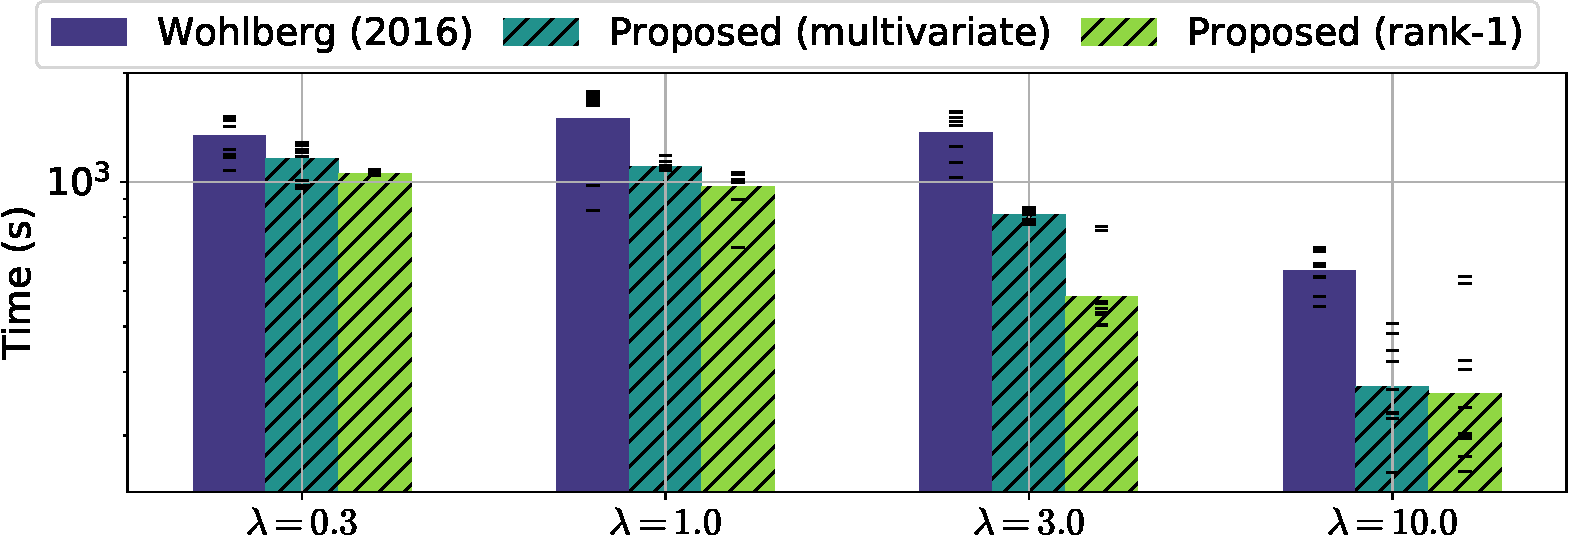
\includegraphics[width=\textwidth]{all_last_0001_T_13470_P5_K8_L128}
\end{frame}


\begin{frame}{Pattern recovery}
Patterns recovered with $P = 1$ and $P=5$. The signals were generated with the two simulated temporal patterns and with  $\sigma = 10^{-3}$. \\[1em]
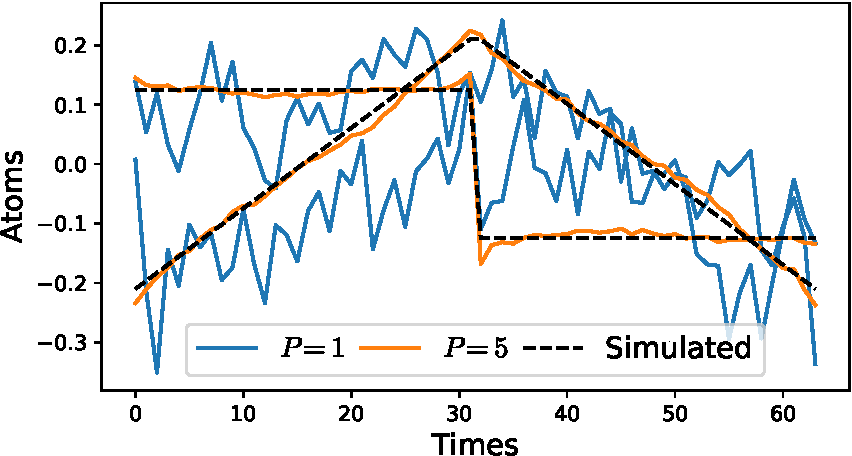
\includegraphics[width=\textwidth]{1D_vs_multi_uv_hat_P5.pdf}
\end{frame}
\begin{frame}{Pattern recovery}
Evolution of the recovery loss with $\sigma$ for different values of $P$. Using more channels improves the recovery of the original patterns.\\[1em]
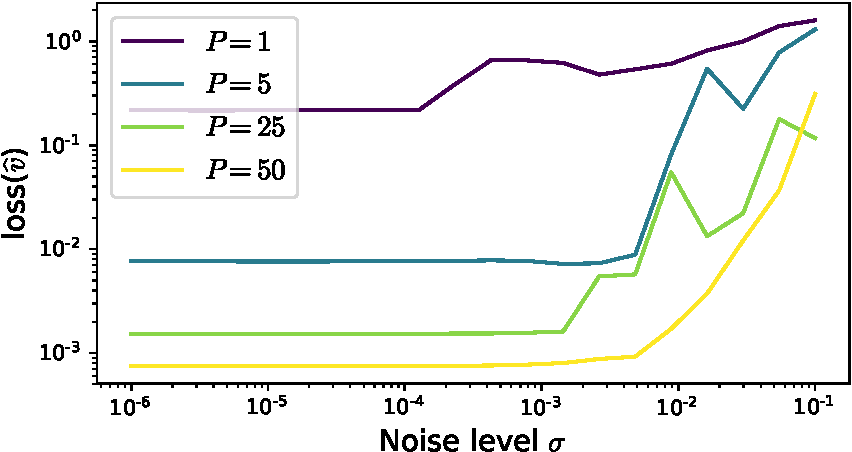
\includegraphics[width=\textwidth]{1D_vs_multi.pdf}
\end{frame}


\section{Experiments on Real Dataset}
\begin{frame}[t]
\vskip5em
\centering
\begin{beamercolorbox}[sep=8pt,center,shadow=true,rounded=true]{title}
	\usebeamerfont{title}\insertsectionhead%
\end{beamercolorbox}
\vskip5em
\flushleft
\large Good time to wake-up if you got lost in the previous section!
\end{frame}

\begin{frame}{MNE somatosensory data}
A selection of temporal waveforms of the atoms learned on the MNE sample dataset.\\
\centering
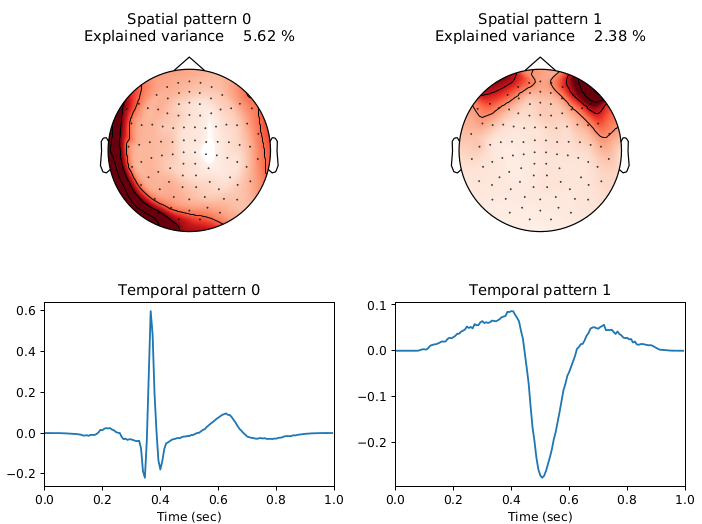
\includegraphics[height=0.8\textheight]{artifacts}
\end{frame}


\begin{frame}{MNE somatosensory data}
Atoms revealed using the MNE somatosensory data. Note the non-sinusoidal comb shape of the mu rhythm.\\[1em]
\centering
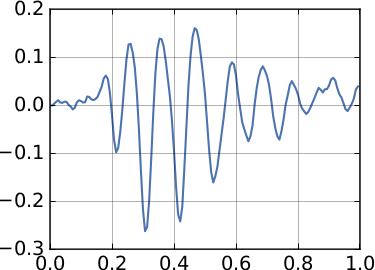
\includegraphics[height=.35\textheight]{atoms_somato_a.png}\hskip3em
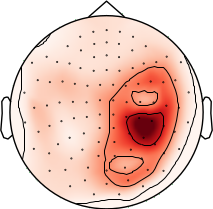
\includegraphics[height=.35\textheight]{atoms_somato_b.png}\\[.3em]\hskip1em
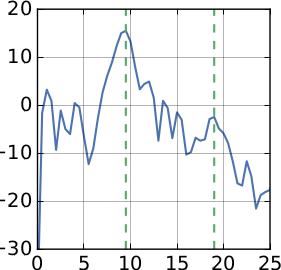
\includegraphics[height=.35\textheight]{atoms_somato_c.png}\hskip3em
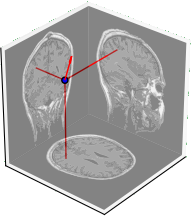
\includegraphics[height=.35\textheight]{atoms_somato_d.png}
\end{frame}


\begin{frame}{Encoding HST images with CDL}
\begin{columns}[c]
    \column{.6\textwidth}
    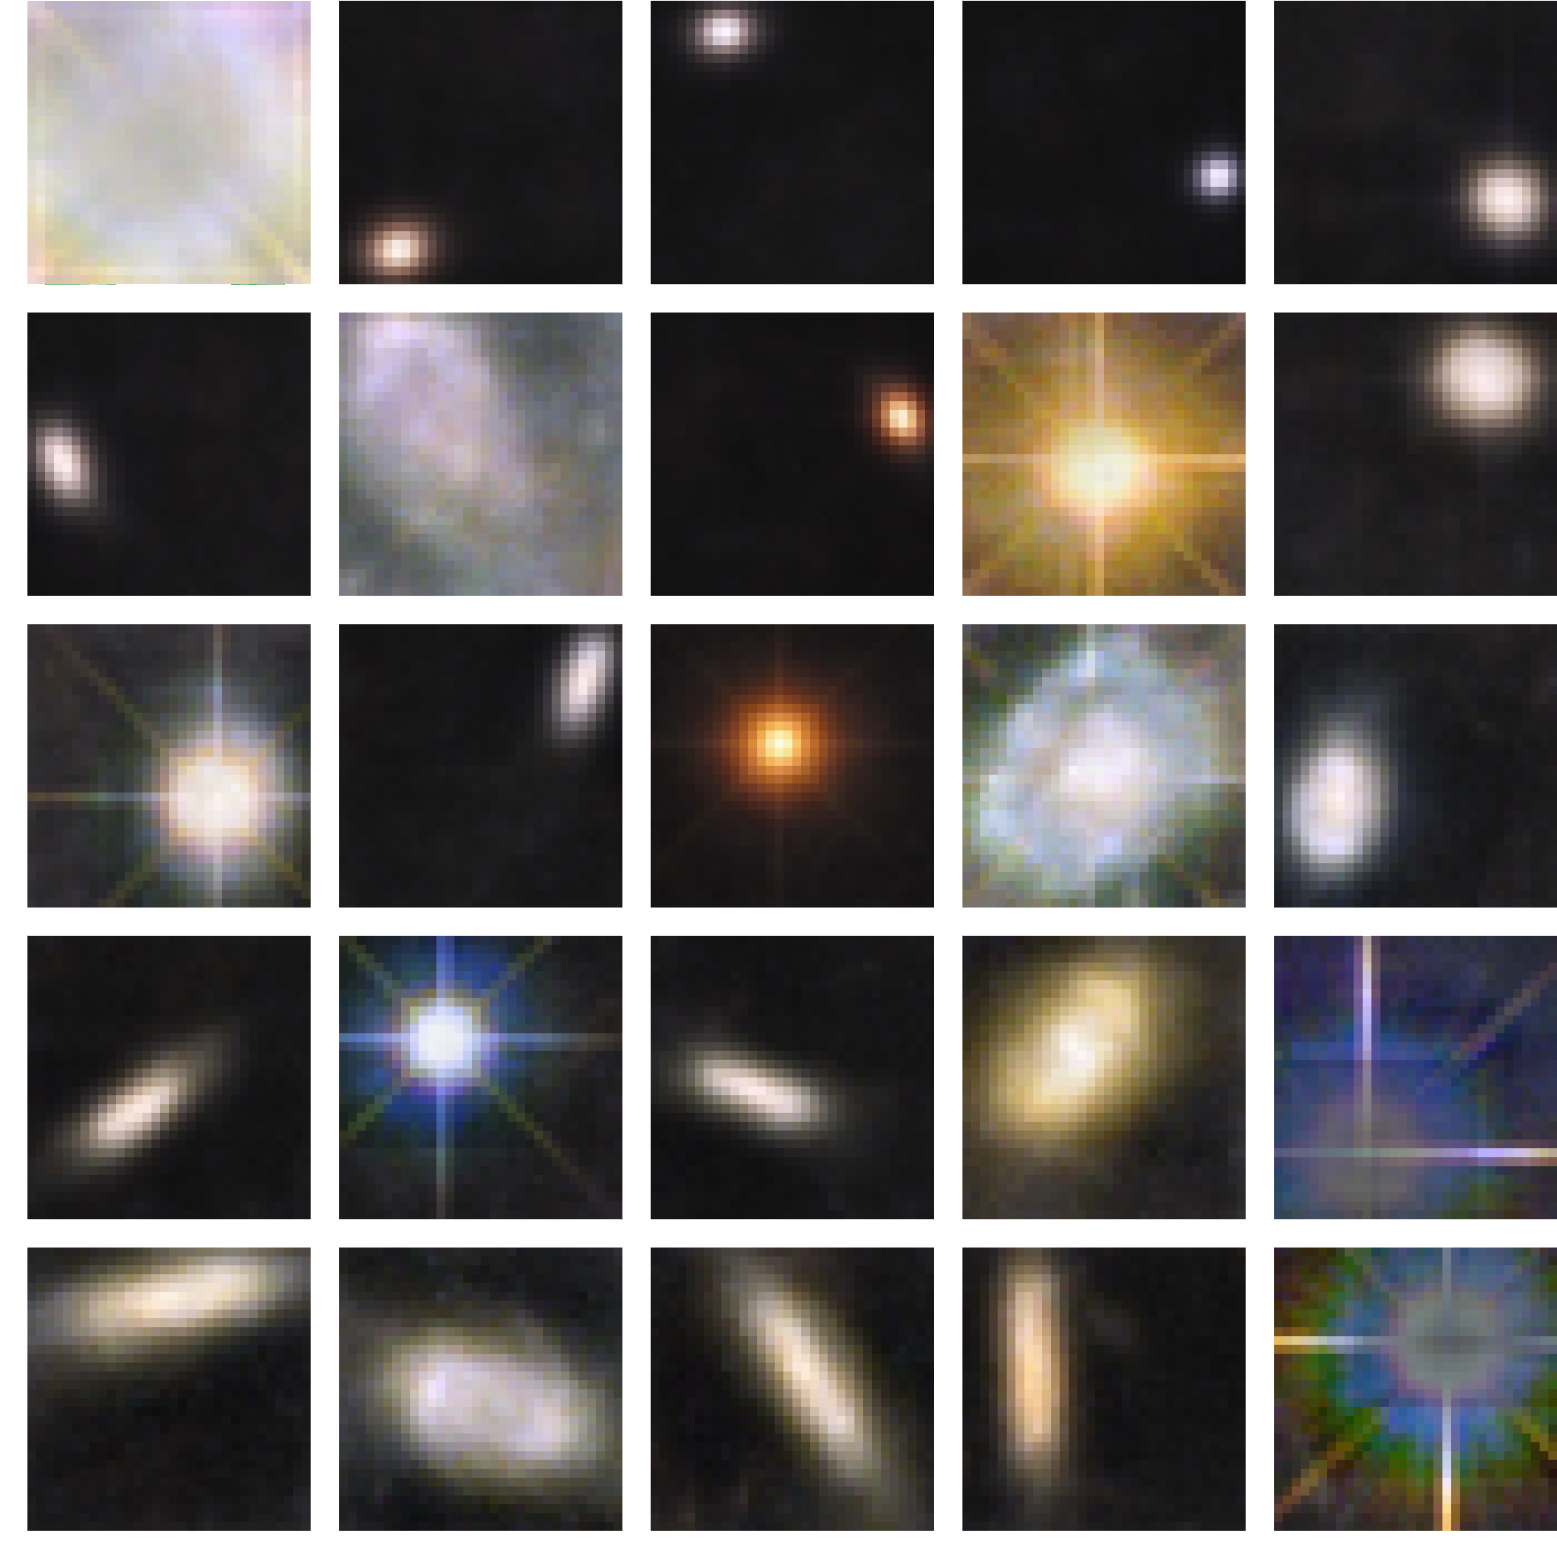
\includegraphics[height=.8\textheight]{K25_L32_reg0,1_seed42_dicodile_Medium_dict.png}
    \column{.4\textwidth}
        Atoms $32\times 32$ learned\\
        with DiCoDiLe on image STScI-H-2016-39-a\\(resolution $6000\times 3664$).\\[1em]
        
        The atoms are order with $\|Z_k\|_1$.
\end{columns}
\end{frame}

\begin{frame}{Conclusion}
\textbf{LGCD and DiCoDile: } Efficient algorithm to scale Convolutional Dictionary Learning to large signals.\\[1.5em]
\textbf{Rank-1 constraints: } Adapt the constraints to the type of patterns researched.\\[2.5em]

\textbf{Ahead of us:}\\[1em]

\begin{itemize}\itemsep1em
    \item Scale invariant atoms?
    \item Pattern detection with extra prior:
\end{itemize}

\end{frame}

\begin{frame}{}
\vskip2em
{\centering
\usebeamercolor[fg]{title}
\usebeamerfont{title}
\Huge \bf Thanks!\\[2em]}

Code available online:\\[1em]
\textbf{alphacsc} : alphacsc.github.io\\[1em]
\textbf{DICOD} (\& DiCoDiLe soon) : github.com/tommoral/dicod\\[3em]

Slides are on my web page:\\[1em]
\hskip5em\includegraphics[height=.8em]{website} tommoral.github.io
\hskip4em 
\includegraphics[height=.8em]{twitter} @tomamoral


\end{frame}


\begin{frame}{Reference}
\tiny
\bibliography{library.bib}
\end{frame}
\end{document}
